20. \begin{figure}[ht!]
\center{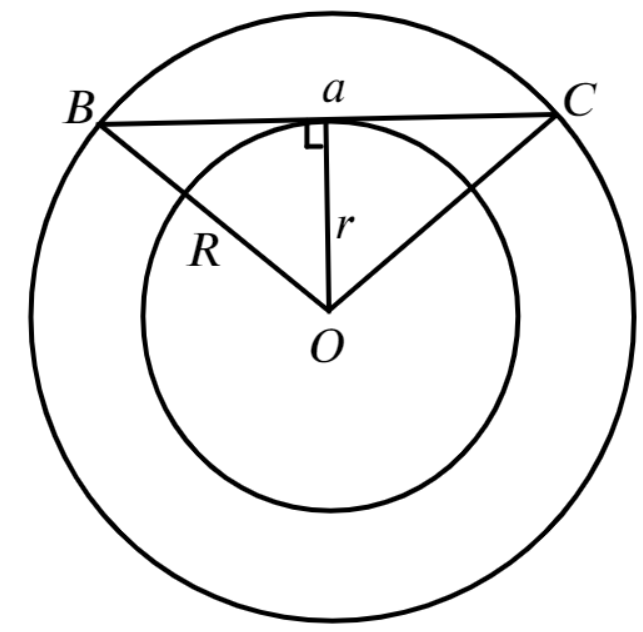
\includegraphics[scale=0.35]{g9-20.png}}
\end{figure}\\
Пусть длина хорды равна $a,$ тогда площадь построенного на ней круга равна $\cfrac{\pi a^2}{4}.$ Если радиусы окружностей равны $R$ и $r,$ то площадь кольца между ними равна $\pi(R^2-r^2).$ Треугольник $OBC$ является равнобедренным ($OB=OC),$ значит в нём высота совпадает с медианой и по теореме Пифагора $R^2-r^2=\cfrac{a^2}{4},$ откуда $\pi(R^2-r^2)=\cfrac{\pi a^2}{4},$ ч.т.д.\\
